% !TeX spellcheck = en_US
\documentclass[letterpaper,12pt,twoside]{report}
\usepackage{fancyhdr}
\usepackage{fullpage}
\usepackage{tikz}
\usepackage{amsmath}

\begin{document}
	\pagestyle{fancy}
	\fancyhf{}
	\fancyhead[L]{Day 13}
	\fancyhead[R]{\textit{The Calendar Project}}
	\fancyfoot[L]{Citations Involved: none}
	
	% Problem
	\paragraph{Problem}
	\begin{quote}
		\textsf{A side length of square $ABCD$
			is 4cm. Use $A$ and the midpoint, $M$,
			of $\overline{CD}$ to form a side of a second
			square. Draw the
			second square,
			$AMEF$, and then
			repeat the process
			using $F$ and $N$, the
			midpoint of $\overline{ME}$, to determine a third
			square, $FNGH$. Find the area of this
			square.}
	\end{quote}
	
	% Graphics
	\begin{center}
		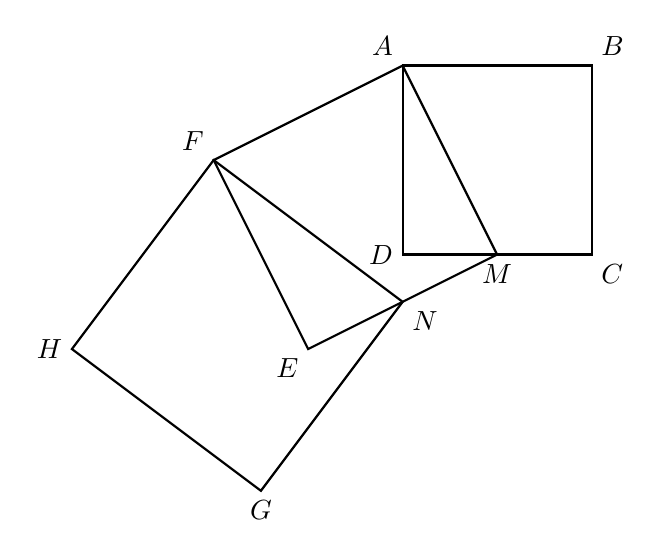
\begin{tikzpicture}[scale=0.6]
		% First square
		\draw[thick] (0,0) -- (4,0) -- (4,4) -- (0,4) -- cycle;
		% Second square
		\draw[thick] (0,4) -- (2,0) -- (-2,-2) -- (-4,2) -- cycle;
		% Third square
		\draw[thick] (-4,2) -- (0,-1) -- (-3,-5) -- (-7,-2) -- cycle;
		
		\node[above left] at (0,4) {$A$};
		\node[above right] at (4,4) {$B$};
		\node[below right] at (4,0) {$C$};
		\node[left] at (0,0) {$D$};
		\node[below] at (2,0) {$M$};
		\node[below left] at (-2,-2) {$E$};
		\node[above left] at (-4,2) {$F$};
		\node[below right] at (0,-1) {$N$};
		\node[below] at (-3,-5) {$G$};
		\node[left] at (-7,-2) {$H$};
		
		\end{tikzpicture}
	\end{center}
	
	% Reasoning
	\paragraph{Reasoning}
	\begin{quotation}
		
		Given that $M$ bisects $\overline{DC}$, $DM=MC$ because $M$ is equidistant to $D$ and $C$ by the definition of segment bisection. Given that the side length of square $ABCD$ is 4 cm, $DC=4$. By the SAP, $DM+MC=DC$. Using substitution and the distributive property, $2DM=DC=4$ and therefore $DM=MC=\frac{4}{2}=2$. Since all internal angles of a square are right angles by definition (1), $\triangle ADM$ is a right triangle. By the Pythagorean Theorem (2), the length of $\overline{AM}$ (the hypotenuse of $\triangle ADM$) is $\sqrt{AD^2+DM^2}=\sqrt{4^2+2^2}=\sqrt{16+4}=\sqrt{20}=2\sqrt{5}$. Since all sides of a square are congruent by definition (1), $2\sqrt{5}=AM=ME=EF=FA$. Using the strategy aforementioned, $EN$ is proven to be $\frac{2\sqrt{5}}{2}=\sqrt{5}$ and $\triangle FEN$ is proven to be a right triangle. By the Pythagorean Theorem (2), $FN=\sqrt{\sqrt{5}^2+(2\sqrt{5})^2}=\sqrt{5+20}=\sqrt{25}=5$, which means that the side length of square $FNGH$ is 5 cm. Using the square area formula $s^2$ where $s$ is the side length of the square, the area of $FNGH$ is determined to be $5^2=\boxed{25\text{  cm}^2}$.
		
	\end{quotation}
	
	\paragraph{External References}
	
	\begin{enumerate}
		\item Textbook Ch. 6, Pg. 410: Definition of a Square
		\item Textbook Ch. 9, Pg. 587: Pythagorean Theorem
	\end{enumerate}
	
\end{document}